\documentclass{article}

% Required packages (merged from hw5_template.tex and hw6_questions.tex)
\usepackage{amssymb}
\usepackage{amsmath}
\usepackage{graphicx}
\usepackage{geometry}
\usepackage{tikz}
\usepackage{array}
\usepackage{booktabs}
\usepackage{enumitem}
\usepackage{listings}
\usepackage{xcolor}
\usepackage{fancyhdr}
\usepackage{float}
\usepackage{subcaption}
\usepackage{comment}
\usepackage{algorithm}
\usepackage{algpseudocode}
\usepackage{caption}
\usepackage{siunitx}
\usepackage{hyperref}
\usetikzlibrary{arrows.meta, positioning} % Required for hw6 diagrams

% Set page geometry
\geometry{a4paper, margin=1in}

% Configure listings for Python
\lstset{
  language=Python,
  basicstyle=\ttfamily\footnotesize,
  numbers=left,
  numberstyle=\tiny\color{gray},
  frame=single,
  breaklines=true,
  breakatwhitespace=true,
  captionpos=b,
  tabsize=4,
  showspaces=false,
  showstringspaces=false,
  showtabs=false,
  commentstyle=\color{gray}\textit,
  keywordstyle=\color{blue}\bfseries,
  stringstyle=\color{red}
}

\begin{document}

\pagestyle{fancy}
\chead{DSC 257: Unsupervised Learning (Fall 2025)}
\lhead{Homework 9}
\rhead{Randall Rogers}

%------------------
% Solution for 1(a)
%------------------
\subsection*{Solution 1}
\noindent\rule{\textwidth}{0.4pt}\\
\subsubsection*{Question 1 (a)}
\begin{flushleft}
    Representations based on clustering Suppose that we have a data set $X=\{x_1, \ldots, x_n\}$ consisting of points in a metric space $(\mathcal{X}, d)$. We cluster the data to get $k$ cluster centers $\mu_1, \ldots, \mu_k \in \mathcal{X}$. Here are a couple of the ways in which we can create a new representation of the data based on this clustering:
\end{flushleft}
\begin{flushleft}
    \textit{Represent each point by its cluster label, i.e., $\phi(x) = \arg \min_j d(x, \mu_j)$.}
\end{flushleft}
\begin{flushleft}
    In each of these cases, precisely specify the space in which the representation $\phi(x)$ lies (e.g. $\mathbb{R}^n$).

Note: When we have a hierarchical clustering, we can get more elaborate multi-scale representations.
\end{flushleft}

\subsubsection*{Solution 1 (a)}

\subsubsection*{\normalfont}{$\therefore$ }

\subsubsection*{Graduate Level Explanation}

\subsubsection*{Learn Fast Explanation}

\noindent\rule{\textwidth}{0.4pt}\\

\newpage

%------------------
% Solution for 1(a)
%------------------
\subsection*{Solution 1}
\noindent\rule{\textwidth}{0.4pt}\\
\subsubsection*{Question 1 (b)}
\begin{flushleft}
    Representations based on clustering Suppose that we have a data set $X=\{x_1, \ldots, x_n\}$ consisting of points in a metric space $(\mathcal{X}, d)$. We cluster the data to get $k$ cluster centers $\mu_1, \ldots, \mu_k \in \mathcal{X}$. Here are a couple of the ways in which we can create a new representation of the data based on this clustering:
\end{flushleft}
\begin{flushleft}
    \textit{Represent each point by its distance to each of the centers, i.e., $\phi(x)_j = d(x, \mu_j)$.}
\end{flushleft}
\begin{flushleft}
    In each of these cases, precisely specify the space in which the representation $\phi(x)$ lies (e.g. $\mathbb{R}^n$).

Note: When we have a hierarchical clustering, we can get more elaborate multi-scale representations.
\end{flushleft}

\subsubsection*{Solution 1 (b)}

\subsubsection*{\normalfont}{$\therefore$ }

\subsubsection*{Graduate Level Explanation}

\subsubsection*{Learn Fast Explanation}

\noindent\rule{\textwidth}{0.4pt}\\

\newpage

%------------------
% Solution for 2
%------------------
\subsection*{Solution 2}
\noindent\rule{\textwidth}{0.4pt}\\
\subsubsection*{Question 2}
\begin{flushleft}
    Each of the following matrices gives distances (not squared distances) between a set of three points. In each case, say whether the distances can be realized in Euclidean space. If they can, show how by specifying three vectors with exactly the given interpoint distances. If they can't, give a reason.

\[
\begin{bmatrix}
0 & 1 & 2 \\
1 & 0 & 1 \\
2 & 1 & 0
\end{bmatrix}, \quad
\begin{bmatrix}
0 & 1 & 3 \\
1 & 0 & 1 \\
3 & 1 & 0
\end{bmatrix}
\]
\end{flushleft}

\subsubsection*{Solution 2}
\begin{flushleft}
    diagonal matrix,symmetric matrices, determinate=0
\end{flushleft}


\subsubsection*{\normalfont}{$\therefore$ }

\subsubsection*{Graduate Level Explanation}

\subsubsection*{Learn Fast Explanation}

\noindent\rule{\textwidth}{0.4pt}\\

\newpage

%------------------
% Solution for 3(a)
%------------------
\subsection*{Solution 3}
\noindent\rule{\textwidth}{0.4pt}\\
\subsubsection*{Question 3 (a)}
\begin{flushleft}
    Consider the following three points in $\mathbb{R}^3$:

\[
x = \begin{bmatrix}1 \\ 2 \\ 3\end{bmatrix}, \quad
y = \begin{bmatrix}-1 \\ 0 \\ 1\end{bmatrix}, \quad
z = \begin{bmatrix}0 \\ -2 \\ -4\end{bmatrix}
\]

\end{flushleft}
\begin{flushleft}
    Let $D$ be the matrix of squared interpoint distances. What is $D$?
    
\end{flushleft}

\subsubsection*{Solution 3 (a)}


\subsubsection*{\normalfont}{$\therefore$ }

\subsection*{Graduate Level Explanation}

\subsection*{Learn Fast Explanation}

\noindent\rule{\textwidth}{0.4pt}\\

\newpage


%------------------
% Solution for 3(b)
%------------------
\subsection*{Solution 3}
\noindent\rule{\textwidth}{0.4pt}\\
\subsubsection*{Question 3 (b)}
\begin{flushleft}
    Consider the following three points in $\mathbb{R}^3$:

\[
x = \begin{bmatrix}1 \\ 2 \\ 3\end{bmatrix}, \quad
y = \begin{bmatrix}-1 \\ 0 \\ 1\end{bmatrix}, \quad
z = \begin{bmatrix}0 \\ -2 \\ -4\end{bmatrix}
\]

\end{flushleft}
\begin{flushleft}

What is the appropriate $H$ matrix for this situation?
  
\end{flushleft}

\subsubsection*{Solution 3 (b)}


\subsubsection*{\normalfont}{$\therefore$ }

\subsection*{Graduate Level Explanation}

\subsection*{Learn Fast Explanation}

\noindent\rule{\textwidth}{0.4pt}\\

\newpage

%------------------
% Solution for 3(c)
%------------------
\subsection*{Solution 3}
\noindent\rule{\textwidth}{0.4pt}\\
\subsubsection*{Question 3 (c)}
\begin{flushleft}
    Consider the following three points in $\mathbb{R}^3$:

\[
x = \begin{bmatrix}1 \\ 2 \\ 3\end{bmatrix}, \quad
y = \begin{bmatrix}-1 \\ 0 \\ 1\end{bmatrix}, \quad
z = \begin{bmatrix}0 \\ -2 \\ -4\end{bmatrix}
\]

\end{flushleft}
\begin{flushleft}

Compute $-\frac{1}{2}HDH$. What do you get?
    
\end{flushleft}

\subsubsection*{Solution 3 (c)}


\subsubsection*{\normalfont}{$\therefore$ }

\subsection*{Graduate Level Explanation}

\subsection*{Learn Fast Explanation}

\noindent\rule{\textwidth}{0.4pt}\\

\newpage

%------------------
% Solution for 3(d)
%------------------
\subsection*{Solution 3}
\noindent\rule{\textwidth}{0.4pt}\\
\subsubsection*{Question 3 (d)}
\begin{flushleft}
    Consider the following three points in $\mathbb{R}^3$:

\[
x = \begin{bmatrix}1 \\ 2 \\ 3\end{bmatrix}, \quad
y = \begin{bmatrix}-1 \\ 0 \\ 1\end{bmatrix}, \quad
z = \begin{bmatrix}0 \\ -2 \\ -4\end{bmatrix}
\]

\end{flushleft}
\begin{flushleft}

Is the answer in (c) the correct Gram matrix for the data?
    
\end{flushleft}

\subsubsection*{Solution 3 (d)}


\subsubsection*{\normalfont}{$\therefore$ }

\subsection*{Graduate Level Explanation}

\subsection*{Learn Fast Explanation}

\noindent\rule{\textwidth}{0.4pt}\\

\newpage

%------------------
% Solution for 4(a)
%------------------
\subsection*{Solution 4}
\noindent\rule{\textwidth}{0.4pt}\\
\subsubsection*{Question 4 (a)}
\begin{flushleft}
    A set of $n$ points in $\mathbb{R}^d$ is orthonormal: that is, each point has unit length and the points are orthogonal to one another.

\end{flushleft}
\begin{flushleft}
    What is the Gram matrix for this data? Be sure to specify its dimension clearly.
    
\end{flushleft}

\subsubsection*{Solution 4 (a)}


\subsubsection*{\normalfont}{$\therefore$ }

\subsection*{Graduate Level Explanation}

\subsection*{Learn Fast Explanation}

\noindent\rule{\textwidth}{0.4pt}\\

\newpage


%------------------
% Solution for 4(b)
%------------------
\subsection*{Solution 4}
\noindent\rule{\textwidth}{0.4pt}\\
\subsubsection*{Question 4 (b)}
\begin{flushleft}
    A set of $n$ points in $\mathbb{R}^d$ is orthonormal: that is, each point has unit length and the points are orthogonal to one another.

\end{flushleft}
\begin{flushleft}

What is the matrix of squared interpoint distances?
  
\end{flushleft}

\subsubsection*{Solution 4 (b)}


\subsubsection*{\normalfont}{$\therefore$ }

\subsection*{Graduate Level Explanation}

\subsection*{Learn Fast Explanation}

\noindent\rule{\textwidth}{0.4pt}\\

\newpage

%------------------
% Solution for 5(a)
%------------------
\subsection*{Solution 5}
\noindent\rule{\textwidth}{0.4pt}\\
\subsubsection*{Question 5 (a)}
\begin{flushleft}
Show the 2-d embedding of the distance matrix obtained by cMDS. Here are the steps to follow:
\begin{itemize}
\item Write a function that implements the classical MDS algorithm from the lecture slides, taking as input a matrix of interpoint distances $D$ and a target embedding dimension $k$.In order
to perform the eigendecomposition, you can use np.linalg.eigh, although note that this
returns eigenvalues in increasing rather than decreasing order.
\item Write a function that takes a 2-d embedding of the points and plots them, annotating each point with the corresponding city name. he function matplotlib.pyplot.annotate is
useful for these annotations.
\end{itemize}
\end{flushleft}

\subsubsection*{Solution 5 (a)}

\subsubsection*{Python Code for d=10}
\begin{lstlisting}
import numpy as np
import matplotlib.pyplot as plt
\end{lstlisting}

\subsubsection*{Plot}
\begin{comment}
\begin{figure}[h]
  
\includegraphics[width=\textwidth]{histogram_d10.png}
  \caption{Histogram of squared lengths for d=10}
\end{figure}
\end{comment}

\subsubsection*{\normalfont}{$\therefore$ }

\noindent\rule{\textwidth}{0.4pt}\\

\newpage

%------------------
% Solution for 5(b)
%------------------
\subsection*{Solution 5}
\noindent\rule{\textwidth}{0.4pt}\\
\subsubsection*{Question 5 (b)}
\begin{flushleft}
he embedding returned by cMDS (or any other multidimensional scaling method) is not unique:
any rotation or translation of the points will produce the same interpoint distances. For this
reason, your plot in (a) is unlikely to correspond to our own map of Europe. Show a rotated
version of points that fits our own map more closely. Here are the steps to follow:
\begin{itemize}
\item Write a function that implements the classical MDS algorithm from the lecture slides, taking as input a matrix of interpoint distances $D$ and a target embedding dimension $k$.In order
to perform the eigendecomposition, you can use np.linalg.eigh, although note that this
returns eigenvalues in increasing rather than decreasing order.
\item Write a function that takes a 2-d embedding of the points and plots them, annotating each point with the corresponding city name. he function matplotlib.pyplot.annotate is
useful for these annotations.
\end{itemize}
\end{flushleft}
\begin{flushleft}
    \item Write a function that takes a 2-d data set and an angle, and rotates each of the points through that angle.
\item Play around with the angle until you find something suitable.
\end{flushleft}
$$
\begin{bmatrix}
    \text{cos}(\theta) & -\text{sin}(\theta) \\
    \text{sin}(\theta) & \text{cos}(\theta) 
\end{bmatrix}
$$
Play around with the angle until you find something suitable.

\subsubsection*{Solution 5 (b)}

\subsubsection*{Python Code}
\begin{lstlisting}
import numpy as np
import matplotlib.pyplot as plt
\end{lstlisting}

\subsubsection*{Plot}
\begin{comment}
\begin{figure}[h]
  
\includegraphics[width=\textwidth]{histogram_d10.png}
  \caption{Histogram of squared lengths for d=10}
\end{figure}
\end{comment}

\subsubsection*{\normalfont}{$\therefore$ }

\noindent\rule{\textwidth}{0.4pt}\\

%------------------
% Solution for 5(c)
%------------------
\subsection*{Solution 5}
\noindent\rule{\textwidth}{0.4pt}\\
\subsubsection*{Question 5 (c)}
\begin{flushleft}
    here are many other algorithms for multidimensional scaling. Some of them work by defining a
“stress function” that captures the disparity between the specified interpoint distances and a given
embedding; this stress function is then minimized using gradient descent. One such approach is
implemented in sklearn.manifold.MDS. Use this to produce an embedding of the distances (use
the setting dissimilarity='precomputed'), and once again find a suitable rotation. Plot the
embedded points, annotated with city names, before and after rotation.
\end{flushleft}

\subsubsection*{Solution 2 (b)}

\subsubsection*{Python Code for d=100}
\begin{lstlisting}
import numpy as np
import matplotlib.pyplot as plt
\end{lstlisting}

\begin{comment}
\begin{figure}[h]
  
\includegraphics[width=\textwidth]{histogram_d100.png}
  \caption{Histogram of squared lengths for d=100}
\end{figure}
\end{comment}

\subsubsection*{\normalfont}{$\therefore$ }

\noindent\rule{\textwidth}{0.4pt}\\

\newpage

%------------------
% Solution for 3
%------------------
\subsection*{Solution 3}
\noindent\rule{\textwidth}{0.4pt}\\
\subsubsection*{Question 3}
\begin{flushleft}
    Suppose $X \in \mathbb{R}^2$ has a Gaussian distribution with mean $\begin{bmatrix}1 \\ 2\end{bmatrix}$ and covariance matrix $\begin{bmatrix}2 & 0 \\ 0 & 4\end{bmatrix}$. 
    What is the distribution of the projection of $X$ onto direction $\frac{1}{\sqrt{2}}\begin{bmatrix}1 \\ 1\end{bmatrix}$? 
\end{flushleft}

\subsubsection*{Solution 3}


\subsubsection*{\normalfont}{$\therefore$ }

\noindent\rule{\textwidth}{0.4pt}\\

\newpage

%------------------
% Solution for 4(a)
%------------------
\subsection*{Solution 4}
\noindent\rule{\textwidth}{0.4pt}\\
\subsubsection*{Question 4 (a)}
\begin{flushleft}
    We have three sensors $(X_1, X_2, X_3)$ whose joint distribution is Gaussian with mean zero and covariance matrix 
    \[
    \begin{bmatrix}
    6 & 3 & 1 \\
    3 & 9 & 0 \\
    1 & 0 & 2
    \end{bmatrix}
    \]
    What is the distribution of sensor $X_3$? 
\end{flushleft}

\subsubsection*{Solution 4 (a)}


\subsubsection*{\normalfont}{$\therefore$ }

\noindent\rule{\textwidth}{0.4pt}\\

\newpage

%------------------
% Solution for 4(b)
%------------------
\subsection*{Solution 4}
\noindent\rule{\textwidth}{0.4pt}\\
\subsubsection*{Question 4 (b)}
\begin{flushleft}
    We have three sensors $(X_1, X_2, X_3)$ whose joint distribution is Gaussian with mean zero and covariance matrix 
    \[
    \begin{bmatrix}
    6 & 3 & 1 \\
    3 & 9 & 0 \\
    1 & 0 & 2
    \end{bmatrix}
    \]
    What is the joint distribution of sensors $X_1, X_2$? 
\end{flushleft}

\subsubsection*{Solution 4 (b)}


\subsubsection*{\normalfont}{$\therefore$ }

\noindent\rule{\textwidth}{0.4pt}\\

\newpage

%------------------
% Solution for 4(c)
%------------------
\subsection*{Solution 4}
\noindent\rule{\textwidth}{0.4pt}\\
\subsubsection*{Question 4 (c)}
\begin{flushleft}
    We have three sensors $(X_1, X_2, X_3)$ whose joint distribution is Gaussian with mean zero and covariance matrix 
    \[
    \begin{bmatrix}
    6 & 3 & 1 \\
    3 & 9 & 0 \\
    1 & 0 & 2
    \end{bmatrix}
    \]
    Suppose we observe $X_2=2$ and $X_3=1$. 
    What is the resulting conditional distribution of $X_1$? 
\end{flushleft}

\subsubsection*{Solution 4 (c)}


\subsubsection*{\normalfont}{$\therefore$ }

\noindent\rule{\textwidth}{0.4pt}\\

\newpage

%------------------
% Solution for 5(a)
%------------------
\subsection*{Solution 5}
\noindent\rule{\textwidth}{0.4pt}\\
\subsubsection*{Question 5 (a)}
\begin{flushleft}
    \textbf{Modeling temperature data with Gaussian processes.} In this question, we will explore modeling of geospatial data via Gaussian processes. 
    Begin by downloading the files \texttt{gptrain.csv} and \texttt{gptest.csv} from the course webpage. 
    Each row in each file corresponds to a temperature reading at a given weather station in Brazil at 2 pm on January 1, 2021. The first column gives the latitude of the station, the second the longitude, and the final column is the temperature reading in degrees Celsius. 
    We will fit a simple Gaussian Process model on \texttt{gptrain.csv} and use it to infer temperatures at other locations at that same date and time. 
    We will fit a Gaussian process with covariance function 
    \[
    k(x, x') = \exp\left(\frac{-\|x-x'\|}{\sigma}\right)
    \]
    and mean function $m(x) = 20$ (degrees Celsius). 
    Here $\|x-x'\|$ denotes Euclidean distance between raw latitude and longitude coordinates. 
    Denote the locations in \texttt{gptrain.csv} by $X_{\text{tr}}$ and the temperatures at those locations by $y_{\text{tr}}$; 
    define $X_{\text{te}}, y_{\text{te}}$ analogously for \texttt{gptest.csv}. Thus $X_{\text{tr}}$ is a $93 \times 2$ matrix while $y_{\text{tr}}$ is a 93-dimensional vector. 
    
    The joint distribution of training and test responses can be written as 
    \[
    \begin{bmatrix} y_{\text{tr}} \\ y_{\text{te}} \end{bmatrix} \sim N\left(\begin{bmatrix} 20 \\ \vdots \\ 20 \end{bmatrix}, \begin{bmatrix} K_{\text{tr}} & K_{\text{tr,te}} \\ K_{\text{te,tr}} & K_{\text{te}} \end{bmatrix}\right)
    \]
    where the block matrix 
    \[
    \begin{bmatrix} K_{\text{tr}} & K_{\text{tr,te}} \\ K_{\text{te,tr}} & K_{\text{te}} \end{bmatrix}
    \]
    is the matrix arising from all pairwise evaluations of the covariance function $k(\cdot)$ over all training and testing locations, and its diagonal components $K_{\text{tr}}$ 
    and $K_{\text{te}}$ are the matrices arising from all pairwise covariances within the training and test sets, respectively. 
    Explain very briefly how the definition of Gaussian process allows us to come to this conclusion. 
\end{flushleft}

\subsubsection*{Solution 5 (a)}


\subsubsection*{\normalfont}{$\therefore$ }

\noindent\rule{\textwidth}{0.4pt}\\

\newpage

%------------------
% Solution for 5(b)
%------------------
\subsection*{Solution 5}
\noindent\rule{\textwidth}{0.4pt}\\
\subsubsection*{Question 5 (b)}
\begin{flushleft}
    \textbf{Modeling temperature data with Gaussian processes.} ... [Intro text from 5(a)  
    
    Define 
    \[
    m_{\text{te}} := \begin{bmatrix} 20 \\ \vdots \\ 20 \end{bmatrix} \in \mathbb{R}^{11}
    \]
    since there are 11 locations in the test set. 
    Using properties of the Gaussian, it can be shown that the distribution of test responses given training locations, training responses, and test locations, follows 
    \[
    y_{\text{te}} \mid y_{\text{tr}}, X_{\text{te}}, X_{\text{tr}} \sim m_{\text{te}} + N\left(K_{\text{te,tr}} \cdot K_{\text{tr}}^{-1}(y_{\text{tr}} - m_{\text{tr}}), K_{\text{te}} - K_{\text{te,tr}} K_{\text{tr}}^{-1} K_{\text{tr,te}}\right)
    \]
    In Bayesian language, this is the posterior predictive distribution. 
    \begin{itemize}
        \item Using $X_{\text{tr}}, X_{\text{te}}$, and $y_{\text{tr}}$, compute the posterior mean of $y_{\text{te}}$ via matrix multiplication, using $\sigma=1.5$ in the covariance function. 
        Report the mean squared error between your computed posterior mean and the true values found in $y_{\text{te}}$. 
        \item Report the mean squared error that you would have obtained by simply predicting the average value in $y_{\text{tr}}$ for all locations. 
    \end{itemize}
\end{flushleft}

\subsubsection*{Solution 5 (b)}

\subsubsection*{Python Code for Posterior Mean and MSE}
\begin{lstlisting}
import numpy as np
import pandas as pd
from scipy.spatial.distance import cdist
\end{lstlisting}

\subsubsection*{\normalfont}{$\therefore$ }

\noindent\rule{\textwidth}{0.4pt}\\

\newpage

%------------------
% Solution for 5(c)
%------------------
\subsection*{Solution 5}
\noindent\rule{\textwidth}{0.4pt}\\
\subsubsection*{Question 5 (c)}
\begin{flushleft}
    \textbf{Modeling temperature data with Gaussian processes.} 
    
    The diagonal of the posterior predictive matrix 
    \[
    K_{\text{te}} - K_{\text{te,tr}} K_{\text{tr}}^{-1} K_{\text{tr,te}}
    \]
    gives the conditional variances of the test responses given $X_{\text{tr}}, X_{\text{te}}$, and $y_{\text{tr}}$. 
    \begin{itemize}
        \item Create a rich grid (at least 5000 points) of test latitudes and longitudes within the range found in the training set. 
        Make a plot showing the predicted (posterior mean) temperature at all points in the grid. 
        You might find the function \texttt{matplotlib.pyplot.imshow} helpful for this. 
        \item Make another plot showing the standard deviation of the prediction at all points in the grid. 
        Plot the locations of the stations found in the training set as well. 
        \item What do you notice about the relationship of the standard deviation of the prediction and the distance of that prediction to a training point? 
    \end{itemize}
\end{flushleft}

\subsubsection*{Solution 5 (c)}

\subsubsection*{Python Code for Grid Predictions and Plots}
\begin{lstlisting}
import numpy as np
import pandas as pd
import matplotlib.pyplot as plt
from scipy.spatial.distance import cdist
\end{lstlisting}

\begin{comment}
\begin{figure}[h]
  \includegraphics[width=\textwidth]{gp_mean_plot.png}
  \caption{Posterior Mean Temperature Grid}
\end{figure}
\begin{figure}[h]
  \includegraphics[width=\textwidth]{gp_std_plot.png}
  \caption{Posterior Standard Deviation Grid}
\end{figure}
\end{comment}

\subsubsection*{\normalfont}{$\therefore$ }

\noindent\rule{\textwidth}{0.4pt}\\

\newpage

%------------------
% Solution for 6(a)
%------------------
\subsection*{Solution 6}
\noindent\rule{\textwidth}{0.4pt}\\
\subsubsection*{Question 6 (a)}
\begin{flushleft}
    \textbf{Four friends} $F_1, F_2, F_3, F_4$ like going to the movies. 
    When a new movie comes out, they behave according to the following scheme: 
    \begin{itemize}
    \item $F_1$ sees the movie with probability 0.5. 
    \item $F_2$ sees the movie with probability 0.7, independently. 
    \item If either of $F_1$ or $F_2$ (or both) see the movie, $F_3$ goes to see it with probability 0.8; 
    if neither $F_1$ nor $F_2$ sees the movie, $F_3$ sees it with probability 0.3. 
    \item If $F_3$ sees the movie, then $F_4$ goes to see it with probability 0.9. 
    If $F_3$ doesn't see the movie, then $F_4$ sees it with probability 0.5. 
    \end{itemize}

    Let $F_1, F_2, F_3, F_4 \in \{0,1\}$ denote who sees the movie. 
    The dependencies between these four random variables can be captured by the following directed graph: 

    \begin{center}
    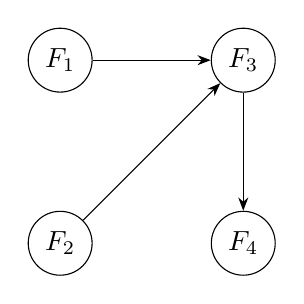
\begin{tikzpicture}[node distance=1.5cm]
        \node[circle, draw] (F1) {$F_1$}; 
        \node[circle, draw, below=of F1] (F2) {$F_2$}; 
        \node[circle, draw, right=of F1] (F3) {$F_3$};
        \node[circle, draw, below=of F3] (F4) {$F_4$};
        \draw[-Stealth] (F1) -- (F3); 
        \draw[-Stealth] (F2) -- (F3); 
        \draw[-Stealth] (F3) -- (F4); 
    \end{tikzpicture}
    \end{center}

    Give the conditional probability tables for this Bayes net. 
\end{flushleft}

\subsubsection*{Solution 6 (a)}


\subsubsection*{\normalfont}{$\therefore$ }

\noindent\rule{\textwidth}{0.4pt}\\

\newpage

%------------------
% Solution for 6(b)
%------------------
\subsection*{Solution 6}
\noindent\rule{\textwidth}{0.4pt}\\
\subsubsection*{Question 6 (b)}
\begin{flushleft}
    \textbf{Four friends} ... [Intro text from 6(a)  

    \begin{center}
    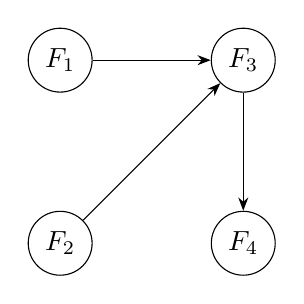
\begin{tikzpicture}[node distance=1.5cm]
        \node[circle, draw] (F1) {$F_1$}; 
        \node[circle, draw, below=of F1] (F2) {$F_2$}; 
        \node[circle, draw, right=of F1] (F3) {$F_3$};
        \node[circle, draw, below=of F3] (F4) {$F_4$};
        \draw[-Stealth] (F1) -- (F3); 
        \draw[-Stealth] (F2) -- (F3); 
        \draw[-Stealth] (F3) -- (F4); 
    \end{tikzpicture}
    \end{center}

    What is the probability of the configuration $F_1 = F_2 = F_3 = 1, F_4 = 0$? 
\end{flushleft}

\subsubsection*{Solution 6 (b)}


\subsubsection*{\normalfont}{$\therefore$ }

\noindent\rule{\textwidth}{0.4pt}\\

\newpage

%------------------
% Solution for 7
%------------------
\subsection*{Solution 7}
\noindent\rule{\textwidth}{0.4pt}\\
\subsubsection*{Question 7}
\begin{flushleft}
    \textbf{Non-uniqueness of underlying DAG.} Suppose random variables $X$ and $Y$ take values in $\{0,1\}$. 
    Does the joint distribution of $(X, Y)$ necessarily factor over the DAG on the left below? 
    What about the DAG on the right? 

    \begin{center}
    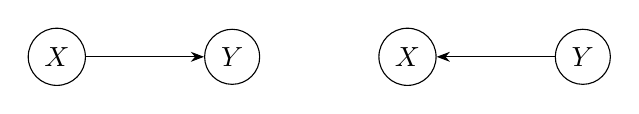
\begin{tikzpicture}[node distance=1.5cm]
        \node[circle, draw] (F1) {$X$}; 
        \node[circle, draw, right=of F1] (F3) {$Y$}; 
        \node[circle, draw, right=of F3] (F2) {$X$};
        \node[circle, draw, right=of F2] (F4) {$Y$};
        \draw[-Stealth] (F1) -- (F3); 
        \draw[-Stealth] (F4) -- (F2); 
    \end{tikzpicture}
    \end{center}
\end{flushleft}

\subsubsection*{Solution 7}


\subsubsection*{\normalfont}{$\therefore$ }

\noindent\rule{\textwidth}{0.4pt}\\

\newpage

%------------------
% Solution for 8(a)
%------------------
\subsection*{Solution 8}
\noindent\rule{\textwidth}{0.4pt}\\
\subsubsection*{Question 8 (a)}
\begin{flushleft}
    \textbf{Genes, diseases, and outcomes.} There is a fictitious disease $(D)$ that can cause paralysis $(P)$. 
    Whether or not an individual gets this disease depends in large part on two genes, $G_1$ and $G_2$. 
    Here is a summary: 

    \begin{itemize}
    \item Each of these genes $G_1, G_2$ can either be normal (also known as wild-type), represented by $G_i=0$, or mutant, represented by $G_i=1$. 
    \item For a person with $G_1=G_2=0$ (both genes wild-type) the probability of acquiring the disease is zero. 
    If $G_1$ is mutant and $G_2$ is wild-type, the probability is 0.2. 
    If $G_1$ is wild-type and $G_2$ is mutant, it is 0.1. 
    And if both genes are mutant, then the disease probability is 0.5. 
    \item For an individual with the disease, the probability of paralysis is 0.5. 
    Without the disease, there is still a small probability of paralysis (from other causes): 0.01. 
    \item $G_1$ is mutant with probability 0.1 and $G_2$ is mutant with probability 0.2; these are independent. 
    \end{itemize}

    Draw a suitable Bayes net over the variables $G_1, G_2, D, P$, and give all relevant conditional probability tables. 
    Let $D=1$ if the disease is present and $D=0$ if it isn't; likewise with paralysis. 
\end{flushleft}

\subsubsection*{Solution 8 (a)}

\subsubsection*{Bayes Net Diagram}
\begin{comment}
    \begin{center}
    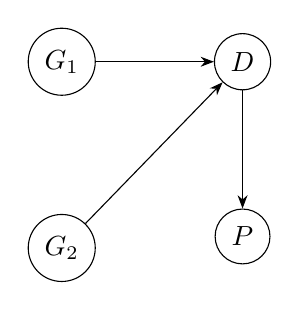
\begin{tikzpicture}[node distance=1.5cm]
        \node[circle, draw] (G1) {$G_1$};
        \node[circle, draw, below=of G1] (G2) {$G_2$};
        \node[circle, draw, right=of G1] (D) {$D$};
        \node[circle, draw, below=of D] (P) {$P$};
        \draw[-Stealth] (G1) -- (D);
        \draw[-Stealth] (G2) -- (D);
        \draw[-Stealth] (D) -- (P);
    \end{tikzpicture}
    \end{center}
\end{comment}

\subsubsection*{Conditional Probability Tables}


\subsubsection*{\normalfont}{$\therefore$ }

\noindent\rule{\textwidth}{0.4pt}\\

\newpage

%------------------
% Solution for 8(b)
%------------------
\subsection*{Solution 8}
\noindent\rule{\textwidth}{0.4pt}\\
\subsubsection*{Question 8 (b)}
\begin{flushleft}
    \textbf{Genes, diseases, and outcomes.} ... [Intro text from 8(a)  

    What is the probability of disease $(D=1)$? 
\end{flushleft}

\subsubsection*{Solution 8 (b)}


\subsubsection*{\normalfont}{$\therefore$ }

\noindent\rule{\textwidth}{0.4pt}\\

\newpage

%------------------
% Solution for 8(c)
%------------------
\subsection*{Solution 8}
\noindent\rule{\textwidth}{0.4pt}\\
\subsubsection*{Question 8 (c)}
\begin{flushleft}
    \textbf{Genes, diseases, and outcomes.} ... [Intro text from 8(a)  

    What is the probability of paralysis $(P=1)$? 
\end{flushleft}

\subsubsection*{Solution 8 (c)}


\subsubsection*{\normalfont}{$\therefore$ }

\noindent\rule{\textwidth}{0.4pt}\\

\newpage

%------------------
% Solution for 8(d)
%------------------
\subsection*{Solution 8}
\noindent\rule{\textwidth}{0.4pt}\\
\subsubsection*{Question 8 (d)}
\begin{flushleft}
    \textbf{Genes, diseases, and outcomes.} ... [Intro text from 8(a)  

    We observe that a person has paralysis. What is the probability that they have the disease? 
\end{flushleft}

\subsubsection*{Solution 8 (d)}


\subsubsection*{\normalfont}{$\therefore$ }

\noindent\rule{\textwidth}{0.4pt}\\

\newpage

%------------------
% Solution for 8(e)
%------------------
\subsection*{Solution 8}
\noindent\rule{\textwidth}{0.4pt}\\
\subsubsection*{Question 8 (e)}
\begin{flushleft}
    \textbf{Genes, diseases, and outcomes.} ... [Intro text from 8(a)  

    We observe that a person has the disease $(D=1)$. 
    What is the probability that they have the mutant form of gene $G_1$? 
\end{flushleft}

\subsubsection*{Solution 8 (e)}


\subsubsection*{\normalfont}{$\therefore$ }

\noindent\rule{\textwidth}{0.4pt}\\

\newpage

%------------------
% Solution for 9(a)
%------------------
\subsection*{Solution 9}
\noindent\rule{\textwidth}{0.4pt}\\
\subsubsection*{Question 9 (a)}
\begin{flushleft}
    \textbf{A character-level RNN for text generation.} Download the file \texttt{rnn-gen.zip} from the course webpage; 
    it contains a Jupyter notebook, \texttt{text-gen-rnn.ipynb}, as well as data and helper files. 
    The notebook is adapted from an excellent blog post by Andrej Karpathy, \textit{The unreasonable effectiveness of recurrent neural networks}. 
    It fits an RNN (more precisely, an LSTM) to the text of Shakespeare's plays and then uses this to generate more text, one character at a time. 
    Work through the notebook and try to understand what is going on. There are just three small questions to answer. 
    
    How many characters are we considering, and what is the integer code for 'A'? 
\end{flushleft}

\subsubsection*{Solution 9 (a)}


\subsubsection*{\normalfont}{$\therefore$ }

\noindent\rule{\textwidth}{0.4pt}\\

\newpage

%------------------
% Solution for 9(b)
%------------------
\subsection*{Solution 9}
\noindent\rule{\textwidth}{0.4pt}\\
\subsubsection*{Question 9 (b)}
\begin{flushleft}
    \textbf{A character-level RNN for text generation.} ... [Intro text from 9(a)  

    What is the length of the corpus in characters? 
\end{flushleft}

\subsubsection*{Solution 9 (b)}


\subsubsection*{\normalfont}{$\therefore$ }

\noindent\rule{\textwidth}{0.4pt}\\

\newpage

%------------------
% Solution for 9(c)
%------------------
\subsection*{Solution 9}
\noindent\rule{\textwidth}{0.4pt}\\
\subsubsection*{Question 9 (c)}
\begin{flushleft}
    \textbf{A character-level RNN for text generation.} ... [Intro text from 9(a)  

    The input and output size for the RNN are set to 66. Why is this? 
\end{flushleft}

\subsubsection*{Solution 9 (c)}


\subsubsection*{\normalfont}{$\therefore$ }

\noindent\rule{\textwidth}{0.4pt}\\

\end{document}
